% Copyright 2004 by Till Tantau <tantau@users.sourceforge.net>.
%
% In principle, this file can be redistributed and/or modified under
% the terms of the GNU Public License, version 2.
%
% However, this file is supposed to be a template to be modified
% for your own needs. For this reason, if you use this file as a
% template and not specifically distribute it as part of a another
% package/program, I grant the extra permission to freely copy and
% modify this file as you see fit and even to delete this copyright
% notice. 

\documentclass[aspectratio=169]{beamer}
%\documentclass{beamer}

\setbeamersize{text margin left=5mm, text margin right=5mm}


\defbeamertemplate{headline}{my header}{%
\vskip1pt%
\makebox[0pt][l]{\,\insertshortauthor}%
\hspace*{\fill}\insertshorttitle/\insertshortsubtitle\hspace*{\fill}%
\llap{\insertpagenumber/\insertpresentationendpage\,}
}
\setbeamertemplate{headline}[my header]

\let\olditem\item
\renewcommand{\item}{\setlength{\itemsep}{\fill}\olditem}

\usepackage{soul}
\usepackage{tkz-euclide}
\usetikzlibrary{calc}
\usepackage[]{algorithm2e}
\usepackage{changepage}
\usepackage{amssymb}
\usepackage{xcolor}
\usepackage{mathtools}
\usepackage{tcolorbox}
\usepackage{tikz}
\usepackage{tikz-3dplot}
\usepackage[export]{adjustbox}
\usepackage{tabu}

% \usepackage[math]{cellspace}
% \cellspacetoplimit 4pt
% \cellspacebottomlimit 4pt
%\usetikzlibrary{arrows.meta}

%\setbeamertemplate{itemize items}{-}

%\usepackage{helvet}
\usefonttheme{professionalfonts} % using non standard fonts for beamer
%\usefonttheme{serif} % default family is serif
%\usepackage{fontspec}
%\setmainfont{Liberation Serif}

% There are many different themes available for Beamer. A comprehensive
% list with examples is given here:
% http://deic.uab.es/~iblanes/beamer_gallery/index_by_theme.html
% You can uncomment the themes below if you would like to use a different
% one:
%\usetheme{AnnArbor}
%\usetheme{Antibes}
%\usetheme{Bergen}
%\usetheme{Berkeley}
%\usetheme{Berlin}
%\usetheme{Boadilla}
%\usetheme{boxes}
%\usetheme{CambridgeUS}
%\usetheme{Copenhagen}
%\usetheme{Darmstadt}
%\usetheme{default}
%\usetheme{Frankfurt}
%\usetheme{Goettingen}
%\usetheme{Hannover}
%\usetheme{Ilmenau}
%\usetheme{JuanLesPins}
%\usetheme{Luebeck}
%\usetheme{Madrid}
%\usetheme{Malmoe}
%\usetheme{Marburg}
%\usetheme{Montpellier}
%\usetheme{PaloAlto}
%\usetheme{Pittsburgh}
%\usetheme{Rochester}
%\usetheme{Singapore}
%\usetheme{Szeged}
%\usetheme{Warsaw}


\def\mf{\ensuremath\mathbf}
\def\mb{\ensuremath\mathbb}
\def\mc{\ensuremath\mathcal}
\def\lp{\ensuremath\left(}
\def\rp{\ensuremath\right)}
\def\lv{\ensuremath\left\lvert}
\def\rv{\ensuremath\right\rvert}
\def\lV{\ensuremath\left\lVert}
\def\rV{\ensuremath\right\rVert}
\def\lc{\ensuremath\left\{}
\def\rc{\ensuremath\right\}}
\def\ls{\ensuremath\left[}
\def\rs{\ensuremath\right]}
\def\bmx{\ensuremath\begin{bmatrix*}[r]}
\def\emx{\ensuremath\end{bmatrix*}}
\def\bmxc{\ensuremath\begin{bmatrix*}[c]}
\def\t{\lp t\rp}
\def\k{\ls k\rs}


\newcommand{\demoex}[2]{\onslide<#1->\begin{color}{black!60} #2 \end{color}}
\newcommand{\demoexc}[3]{\onslide<#1->\begin{color}{#2} #3 \end{color}}
\newcommand{\anim}[3]{\onslide<#1->{\begin{color}{#2!60} #3 \end{color}}}
\newcommand{\ct}[1]{\lp #1\rp}
\newcommand{\dt}[1]{\ls #1\rs}
\newcommand{\cols}[2]{\begin{columns}[#1] #2 \end{columns}}
\newcommand{\col}[2]{\begin{column}{#1} #2 \end{column}}

\newcommand{\xdownarrow}[1]{%
  {\left\downarrow\vbox to #1{}\right.\kern-\nulldelimiterspace}
}

\title{Introduction to Digital Signal Processing}

% A subtitle is optional and this may be deleted
\subtitle{Fourier Representation of Continuous-Time Signals}

\author{Sivakumar Balasubramanian}
% - Give the names in the same order as the appear in the paper.
% - Use the \inst{?} command only if the authors have different
%   affiliation.

\institute[Christian Medical College] % (optional, but mostly needed)
{
  \inst{}%
  Department of Bioengineering\\
  Christian Medical College, Bagayam\\
  Vellore 632002
}
% - Use the \inst command only if there are several affiliations.
% - Keep it simple, no one is interested in your street address.

\date{}
% - Either use conference name or its abbreviation.
% - Not really informative to the audience, more for people (including
%   yourself) who are reading the slides online

\subject{Lecture slides on Introduction to DSP}
% This is only inserted into the PDF information catalog. Can be left
% out. 

% If you have a file called "university-logo-filename.xxx", where xxx
% is a graphic format that can be processed by latex or pdflatex,
% resp., then you can add a logo as follows:

% \pgfdeclareimage[height=0.5cm]{university-logo}{university-logo-filename}
% \logo{\pgfuseimage{university-logo}}

% Delete this, if you do not want the table of contents to pop up at
% the beginning of each subsection:
\AtBeginSubsection[]
{
  \begin{frame}<beamer>{Outline}
    \tableofcontents[currentsection,currentsubsection]
  \end{frame}
}

% Let's get started
\begin{document}

\begin{frame}
  \titlepage
\end{frame}


\begin{frame}[t]{Representation of signals as a linear combination of other signals}
  \begin{itemize}
    \item Decomposition of an object into smaller/simpler components is a useful operation.

     \item Decomposing $x[n]$ as a $\sum_{k=-\infty}^{\infty} x[k] \delta[n - k]$ was useful in understanding input-output relationship of LTI systems.

     \item Infinitely many ways of decomposing a signal.

     \item Decomposing into complex exponential signals is one of the oldest, most common, and very useful approaches $\longrightarrow$ \textbf{Fourier analysis}.
  \end{itemize}
\end{frame}


\begin{frame}[t]{An example from Optics}
  \begin{figure}
  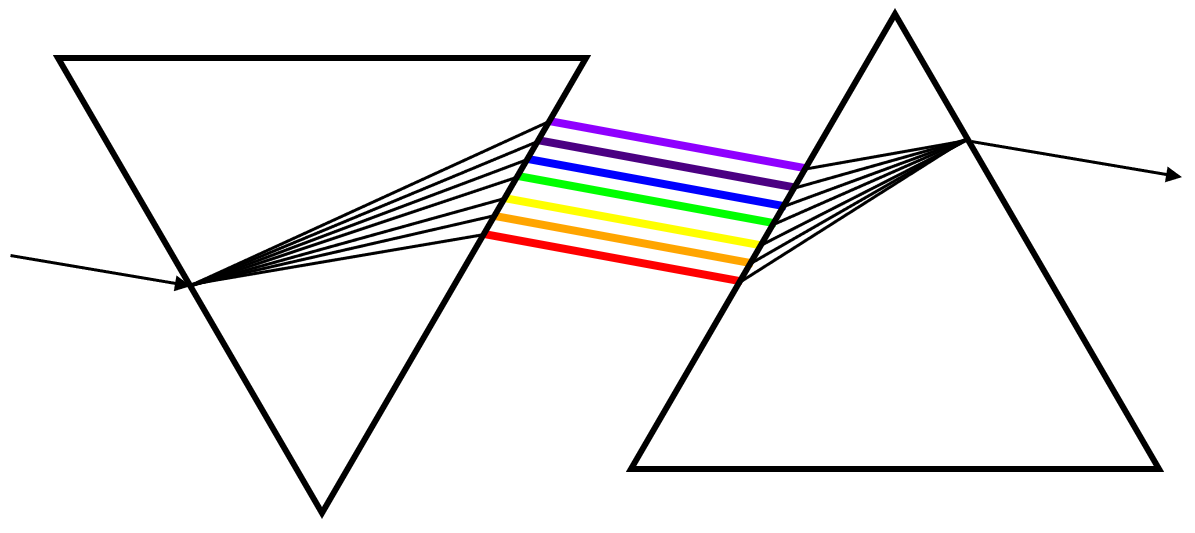
\includegraphics[width=0.6\textwidth]{img/decomp.png}
  \end{figure}

  \begin{itemize}
    \item Sunlight (white light) can be decomposed into different colors using a prism.

    \item Individual colors can be cobmined to produce white light back.
  
    \item Using a filter between the two prisms will allow us to mix the individual colors in different combinations.
  \end{itemize}
\end{frame}

\begin{frame}[t]{Spectral analysis of signals}
  \begin{itemize}
    \item Signals can be decomposed into different sinusoidal components.

    \item Each sinusoidal component is index or parametrized by its frequency.

    \item Let the set of all sinusoidal signals be $S_{ct} = \left\{ s_{\omega}\lp t \rp \vert \,\, \omega \in \mb{R} \right\}$ for continous-time signals, or $S_{dt} = \left\{ s_{\Omega}\ls n \rs \vert \,\, \Omega \in \left( -\pi , \pi\right] \right\}$ for discrete-time singals.
    \[ x\lp t \rp = \int_{-\infty}^{\infty} X\lp \omega \rp s_\omega\lp t \rp d\omega \quad \quad \quad y\ls n \rs = \int_{-\pi}^{\pi} Y\lp \Omega \rp s_\Omega\ls n \rs d\Omega \]

    $X\lp \omega \rp$ is the ``amount'' of $s_{\omega}\lp t \rp$ present in $x\lp t \rp$.

    $Y\lp \Omega \rp$ is the ``amount'' of $s_{\Omega}\ls n \rs$ present in $y\ls n \rs$.    
  \end{itemize}
\end{frame}


\begin{frame}[t]{Fourier Series: Linear combination of periodic signals}
\begin{itemize}
  \item Consider the following set of sinusoidal signals $\left\{ \sin\lp k\cdot \omega_0 t\rp \,\, \vert \,\, k \in \mb{Z}_{>0} \right\}$.
  
  \item $\omega_0 = 2 \pi f_0 = 2\pi\frac{1}{T_0}$ is the fundamental angular frequency of the sinusoidal signal $\sin \lp \omega_0 t \rp$.

  \item Any singal of the following signal will be periodic.
  \[ x\lp t \rp = r_0 + \sum_{k=1}^{\infty} r_k \sin\lp k\cdot \omega_0 t + \phi_k \rp, \,\,\, 0 \leq r_k \in \mb{R}, \,\, \phi_k \in \lp -\pi, \pi \rs \]
  \vspace{0.25cm}
  What is the fundamental period of the signal?
\end{itemize}
\end{frame}


\begin{frame}[t]{Fourier Series: Linear combination of periodic signals}
\begin{itemize}
  \item We can generate new periodic signals (of fundamental frequency $f_0$) by mixing sinusoidal signals with fundamental frequencies that are integer multiples of $f_0$.
  \[ x\lp t \rp = r_0 + \sum_{k=1}^{\infty} r_k \sin\lp k\cdot \omega_0 t + \phi_k \rp, \,\,\, 0 \leq r_k \in \mb{R}, \,\, \phi_k \in \lp -\pi, \pi \rs \]
\end{itemize}
\vspace{-0.2cm}
\begin{figure}
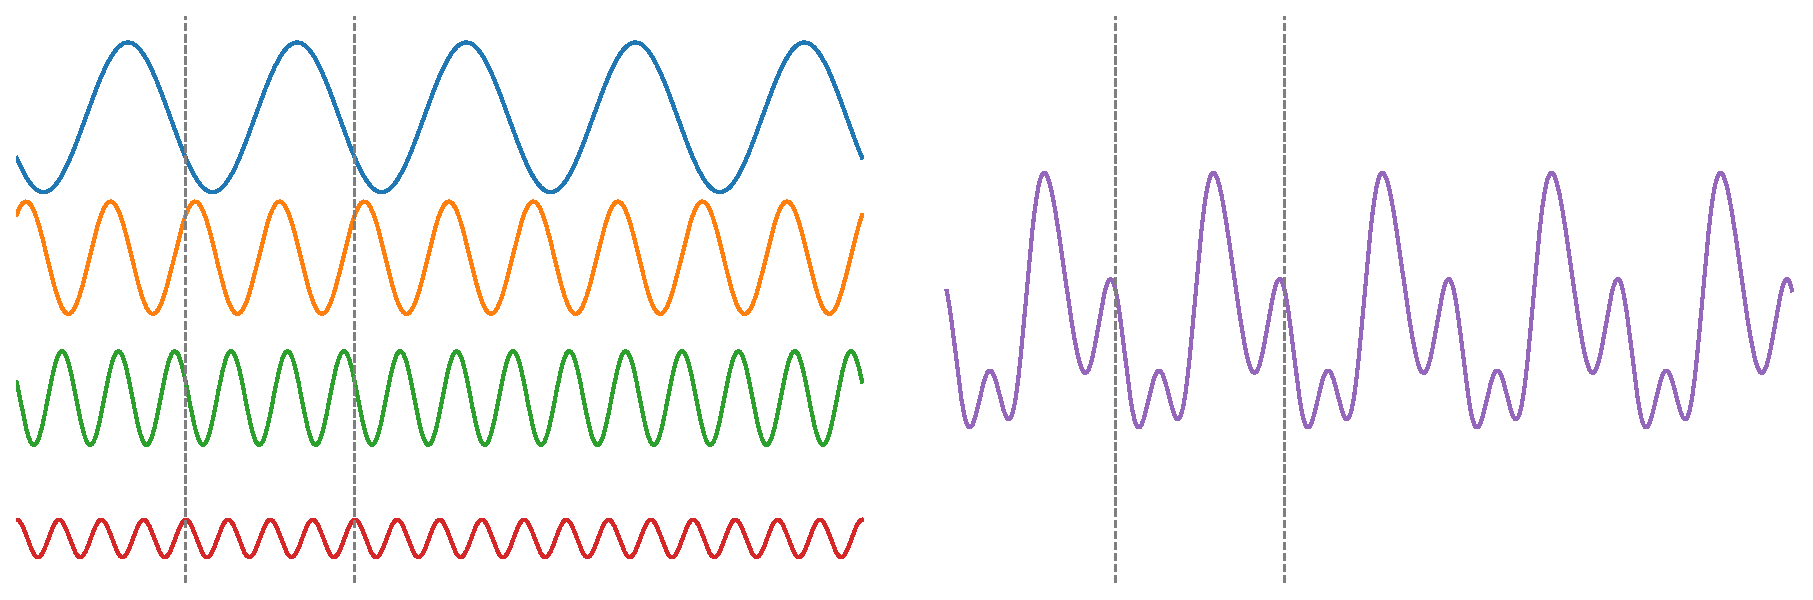
\includegraphics[width=0.9\textwidth]{img/sinesums.eps}
\end{figure}
\end{frame}


\begin{frame}[t]{Fourier Series}
\[ \begin{split}
    x\lp t \rp &= r_0 + \sum_{k=1}^{\infty} r_k \sin\lp k\cdot \omega_0 t + \phi_k \rp \\
    &= r_0 + \sum_{k=1}^{\infty} a_k \sin\lp k\cdot \omega_0 t\rp + b_k \cos\lp k\cdot \omega_0 t\rp\\
    &= \sum_{k=0}^{\infty} \lp a_k \sin\lp k\cdot \omega_0 t\rp + b_k \cos\lp k\cdot \omega_0 t\rp \rp\\
    \end{split}
  \]
Expressing $\cos(\cdot)$ and $\sin(\cdot)$ in terms of complex exponentials, and grouping terms together,
\[ x\lp t \rp = \sum_{k=-\infty}^{\infty} c_k e^{j2\pi k f_0 t} \]
\end{frame}


\begin{frame}[t]{Fourier Series}
\[ x\lp t \rp = \sum_{k=-\infty}^{\infty} c_k e^{j2\pi k f_0 t} \]

Knowing $f_0$, we can compute the signal $x\lp t \rp$ from the list of numbers $(c_k)_{k=-\infty}^{\infty}$.

\vspace{1cm}

We can compute $c_k$ as the following,
\[ c_k = \frac{1}{T_0} \int_{0}^{T_0} x\lp t \rp e^{-j2\pi k f_0 t} dt \]
\end{frame}


\begin{frame}[t]{Fourier Series}
\begin{figure}
  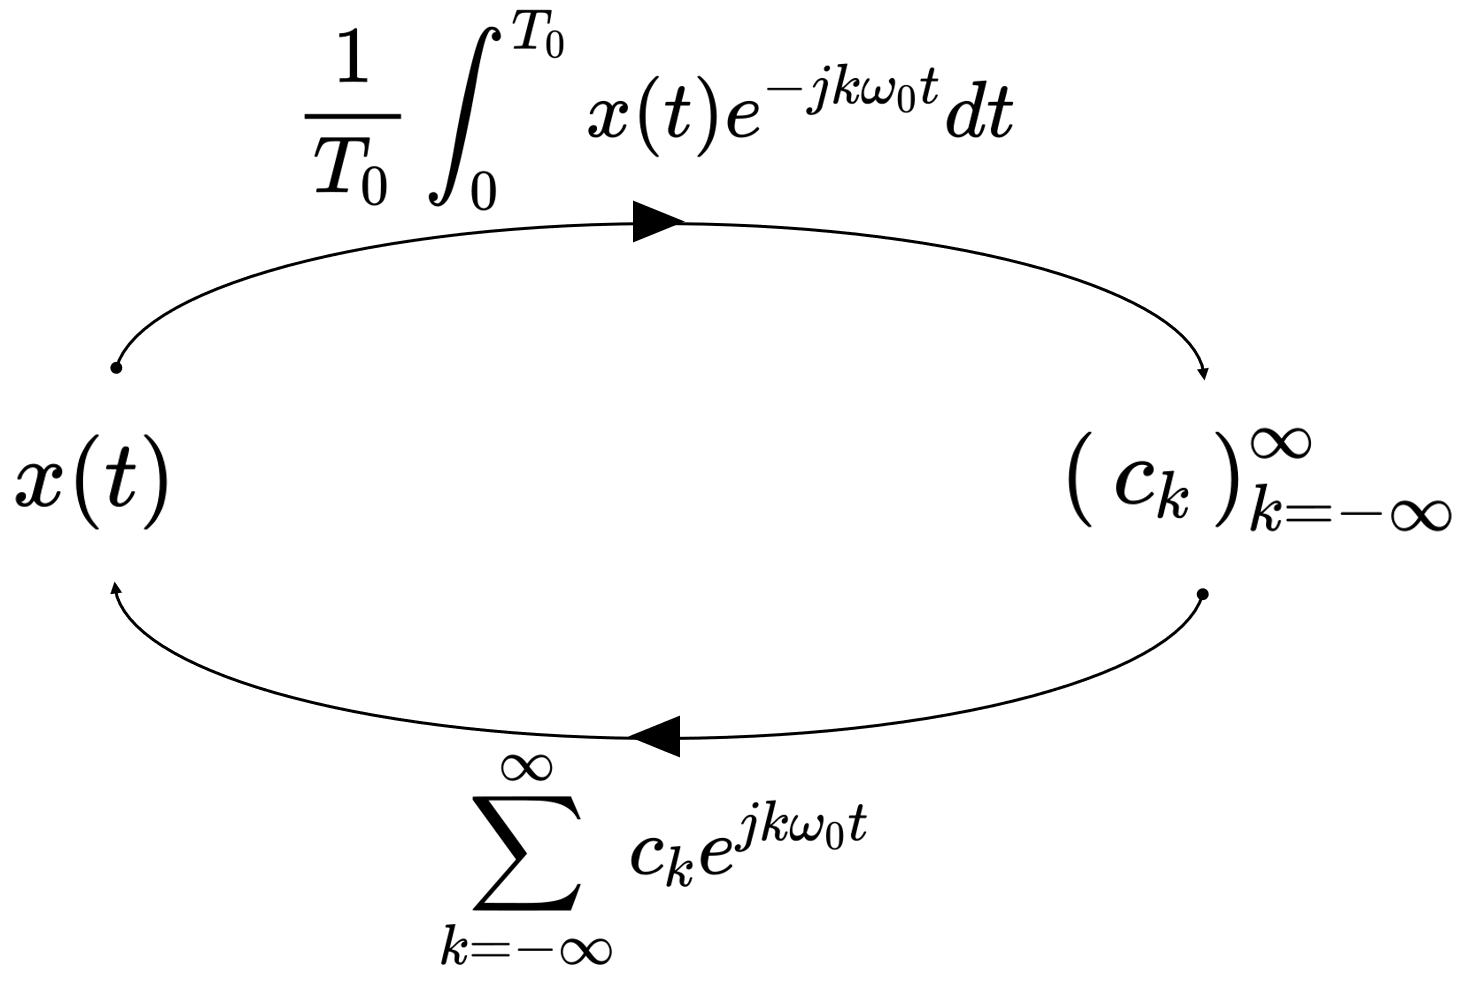
\includegraphics[width=0.7\textwidth]{img/fourierseries.png}
\end{figure}
\end{frame}


\begin{frame}[t]{Fourier Series}
\begin{figure}
  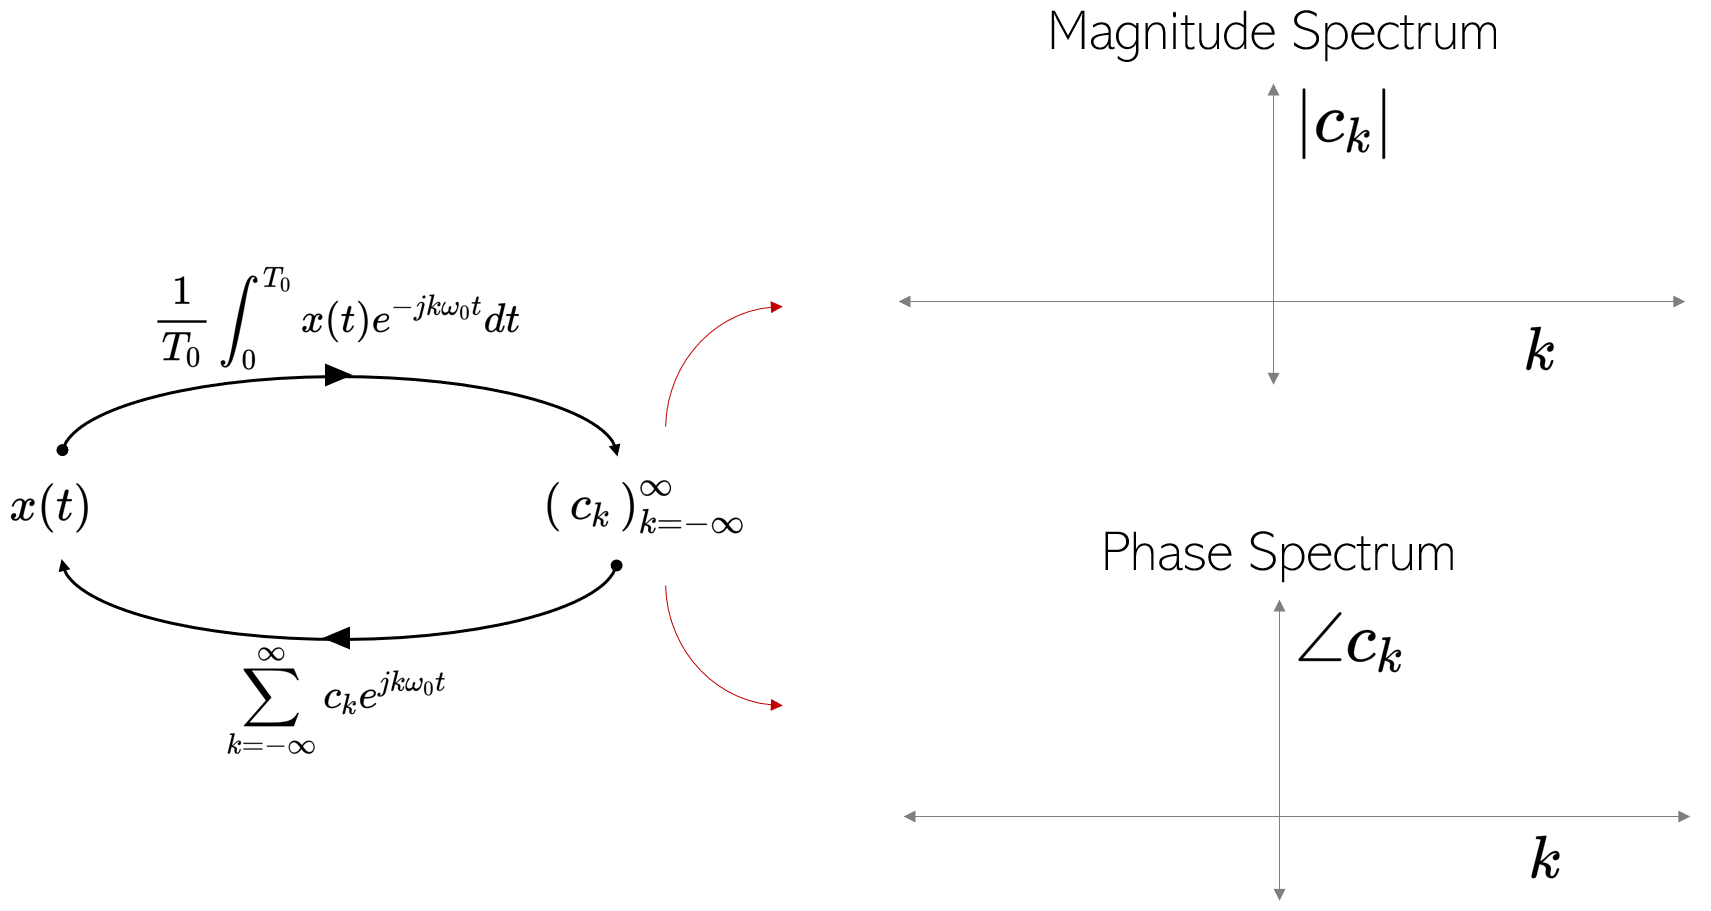
\includegraphics[width=0.9\textwidth]{img/fsspectrum.png}
\end{figure}
\end{frame}


\begin{frame}[t]{Fourier Series}
\vspace{-0.5cm}
\begin{small}
\[ x(t) = -0.1 + 0.8 \cos\lp 2\pi t\rp + 0.5 \cos\lp 4\pi t + \frac{\pi}{4}\rp + 0.05 \cos\lp 6\pi t - \frac{\pi}{4}\rp + 0.2 \cos\lp 8\pi t + \frac{8\pi}{9}\rp \]
\end{small}

\begin{figure}
  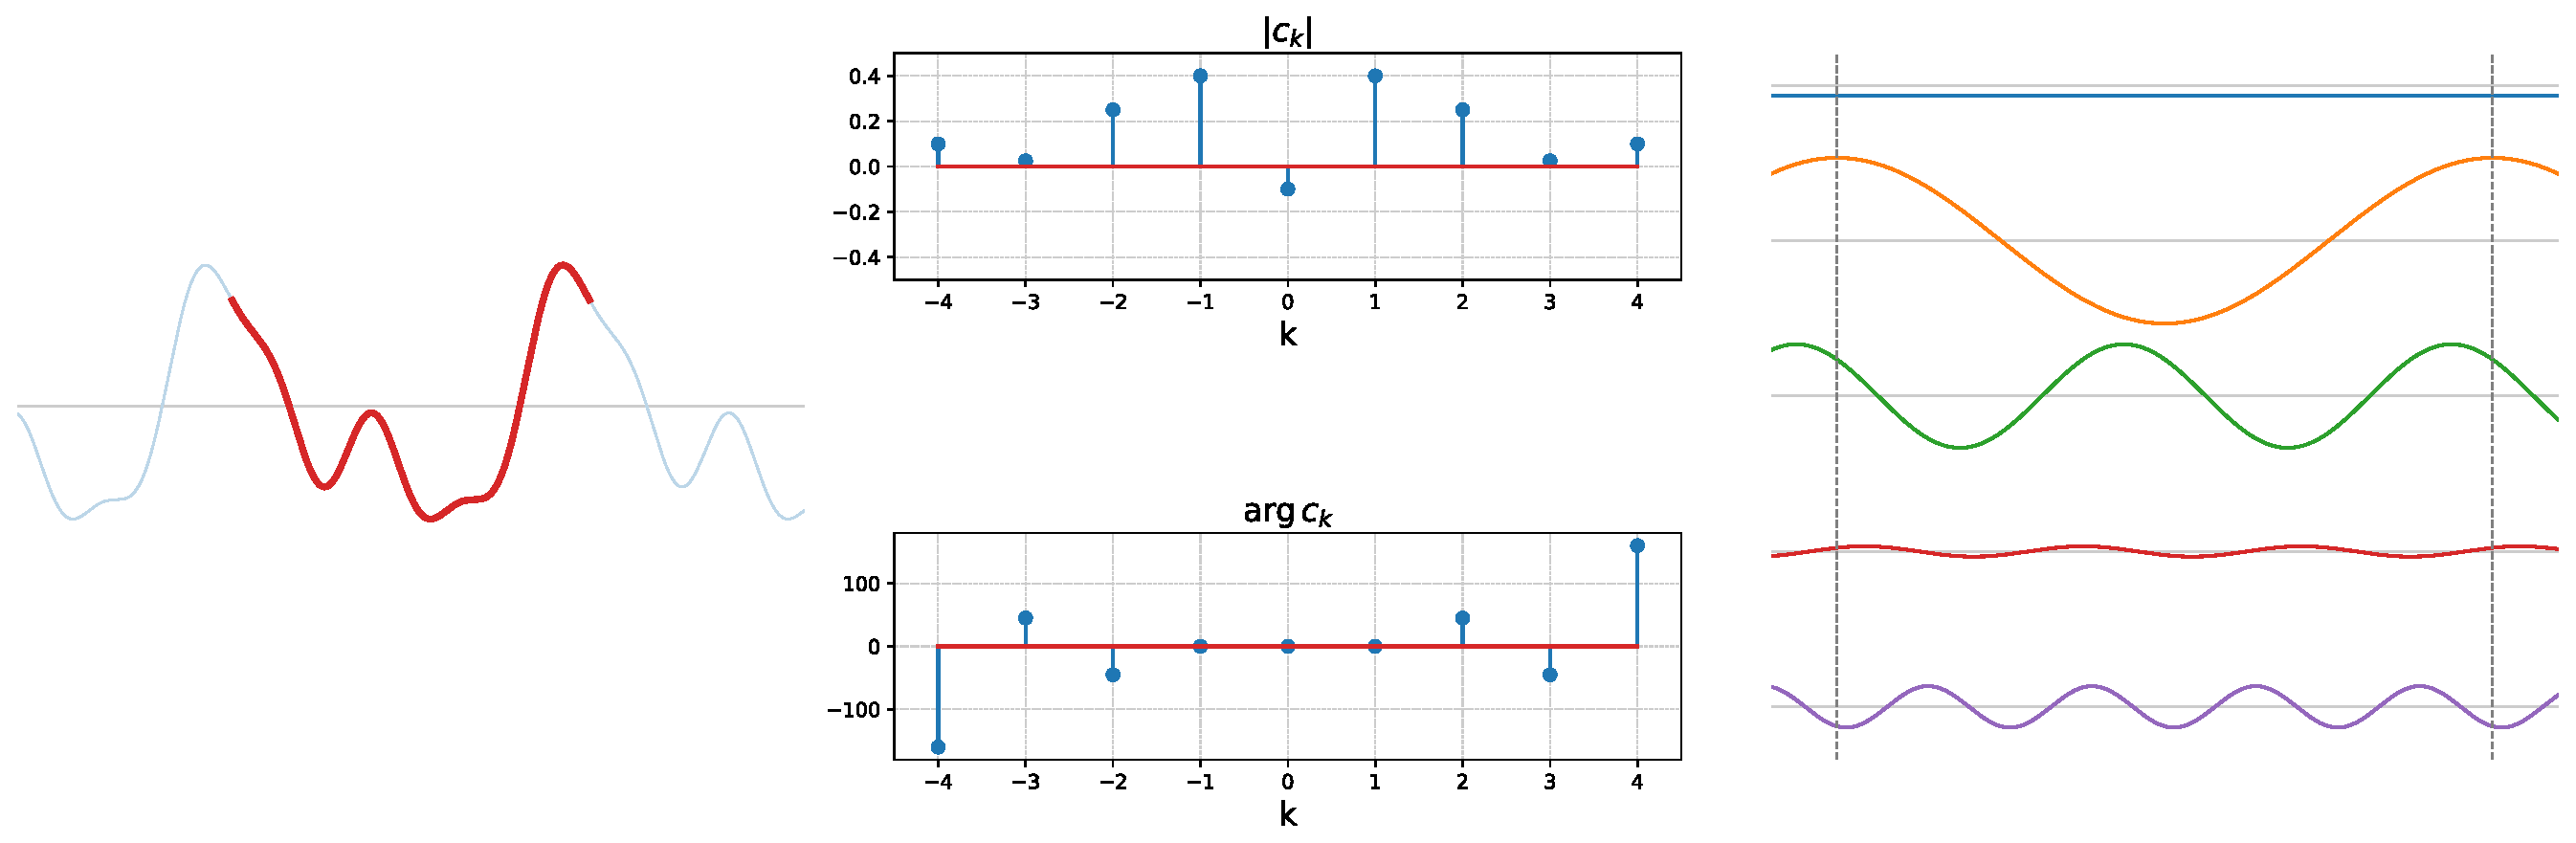
\includegraphics[width=1.0\textwidth]{img/fs-demo.eps}
  \end{figure}
\end{frame}


\begin{frame}[t]{Fourier Series}
\vspace{-0.5cm}
\begin{small}
\[ x(t) = 0.8 \sin\lp 2\pi t\rp + 0.5 \sin\lp 4\pi t + \frac{\pi}{4}\rp + 0.05 \sin\lp 6\pi t - \frac{\pi}{4}\rp + 0.2 \sin\lp 8\pi t + \frac{8\pi}{9}\rp \]
\end{small}

\begin{figure}
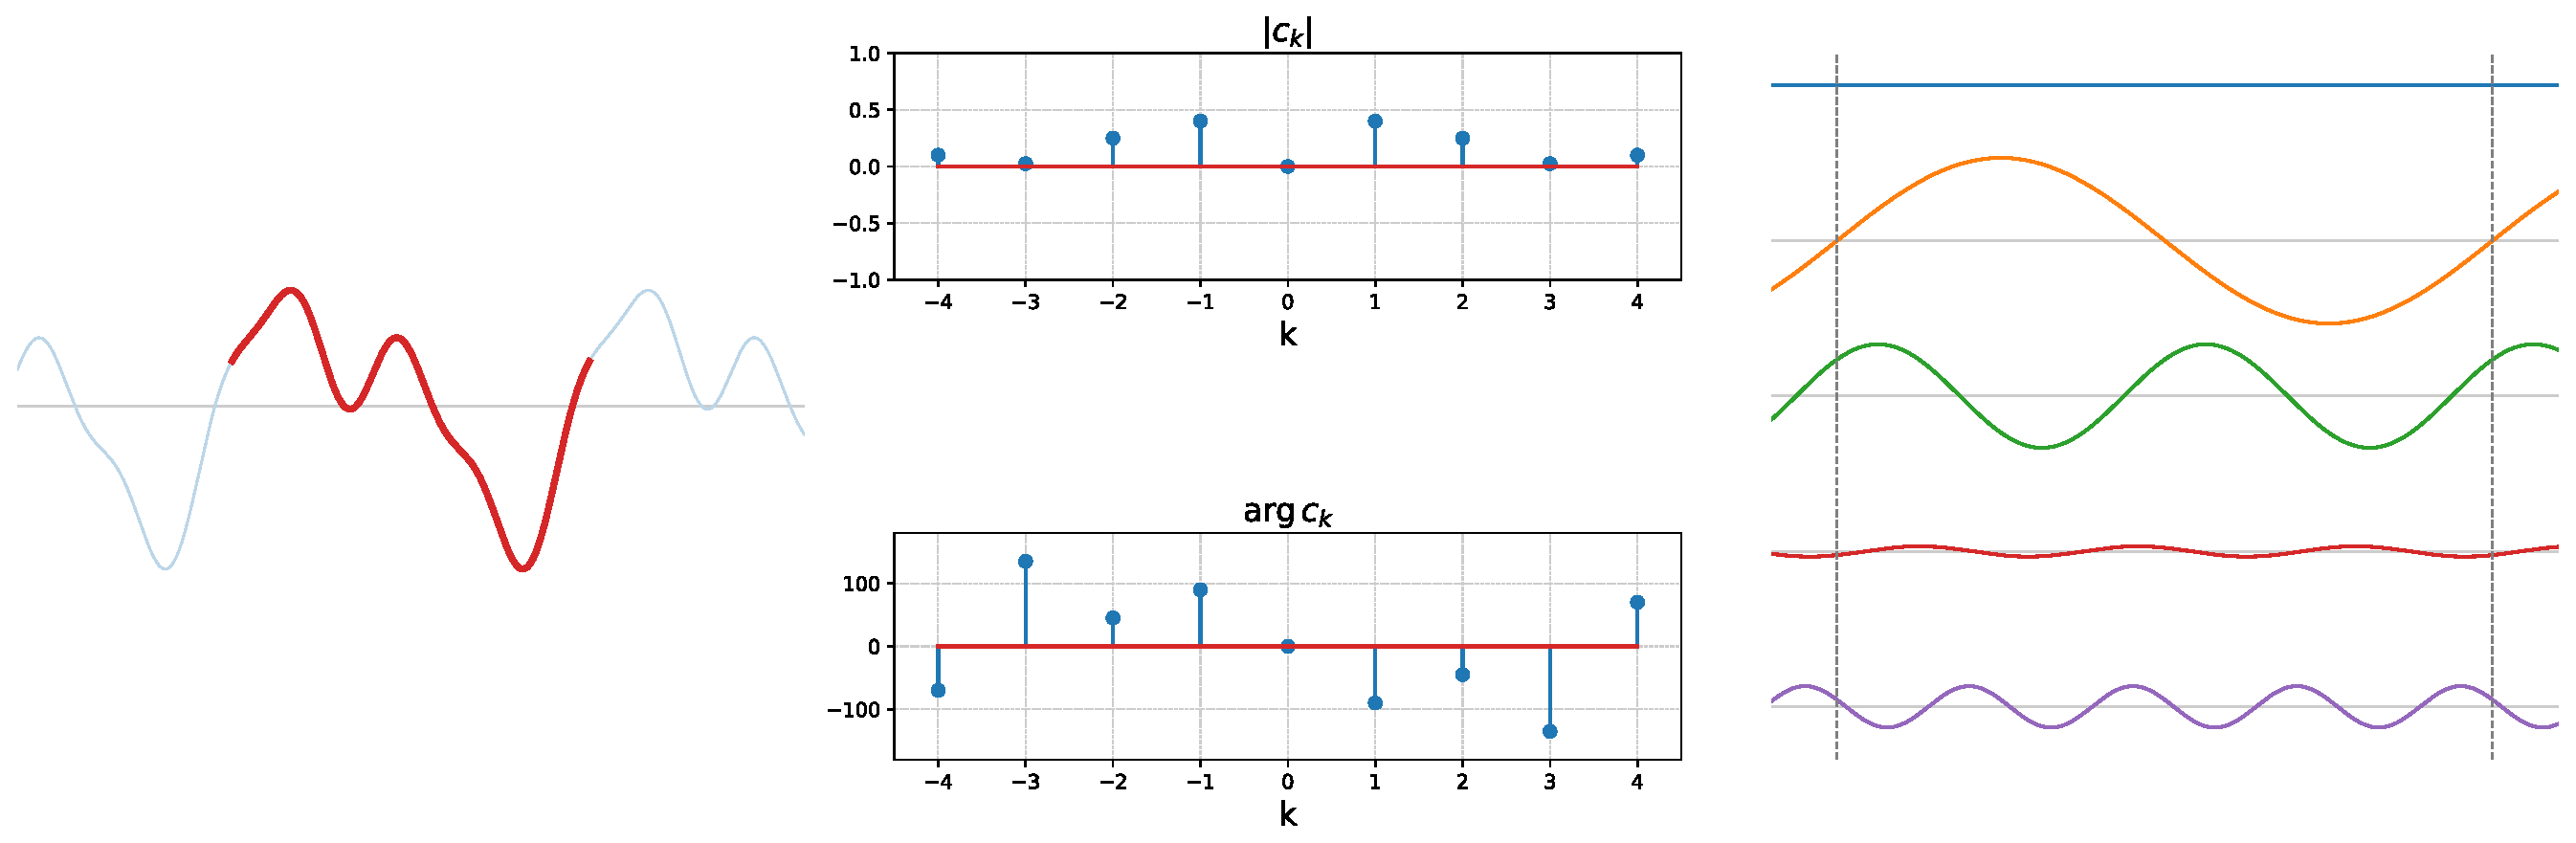
\includegraphics[width=1.0\textwidth]{img/fs-demo-sin.eps}
\end{figure}
\end{frame}


\begin{frame}[t]{Does any periodic signal have a Fourier series representation?}
\begin{itemize}
  \item If $x(t)$ is absolutely integrable over a single cycle, then the Fourier serious coefficients exist.
  \item Any continuous periodic function will have a Fourier series representation.

  \item When $x(t)=$ is continuous and finite, then reconstructed signal $\sum_{k=-\infty}^{\infty} c_k e^{-jk \omega_0 t}$ will be equal to $x(t)$ pointwise.
  \[ x\lp t \rp = \sum_{k=-\infty}^{\infty} c_k e^{-jk \omega_0 t} \,\,\ \forall t \]
\end{itemize}
\end{frame}


\begin{frame}[t]{Does any periodic signal have a Fourier series representation?}
\vspace{-0.5cm}
% \begin{small}
\[ x(t) = \begin{cases} t, & 0 \leq t < 0.5 \\
1 - t, & 0.5 \leq t < 1\end{cases} \,\, \longrightarrow \,\, c_k = \begin{cases} \frac{1}{4}, & k = 0 \\ \frac{4}{k^2\omega_0^2}\sin^2\lp \frac{k \omega_0}{4} \rp e^{-j\frac{k \omega_0}{2}},  & k \neq 0 \end{cases} \]
% \end{small}

\begin{figure}
  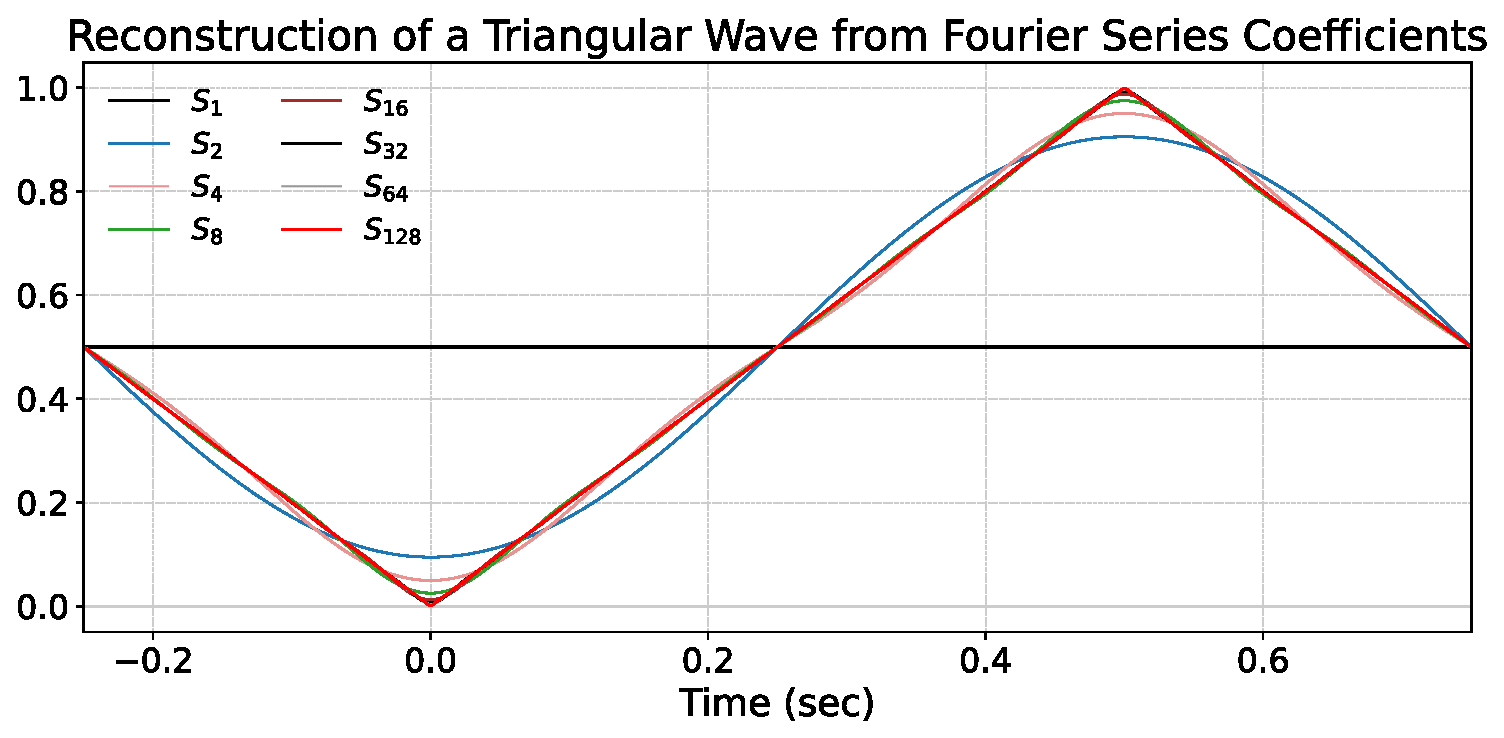
\includegraphics[width=0.8\textwidth]{img/fs-triwave.eps}
  \end{figure}
\end{frame}


\begin{frame}[t]{Does any periodic signal have a Fourier series representation?}
\begin{itemize}
  \item If $x(t)$ is finite but discontinuous $\longrightarrow$ No pointwise equality. Only means squared convergence is possible.
  \[ \lim_{N \to \infty} \int_{0}^{T_0}\left|x(t) - \sum_{k=-N}^{N} c_k e^{j2\pi k f_0 t} \right|^2dt = 0 \]
  This means that the reconstructed signal $\sum_{k=-N}^{N} c_k e^{j2\pi k f_0 t}$ need not be equal to the signal $x(t)$ at a discrete set of points, i.e. at the points where there is a discontinuity.
\end{itemize}
\end{frame}


\begin{frame}[t]{Does any periodic signal have a Fourier series representation?}
\vspace{-0.5cm}
% \begin{small}
\[ x(t) = \begin{cases} 1, & 0 \leq t < 0.5 \\
0, & 0.5 \leq t < 1\end{cases} \,\, \longrightarrow \,\, c_k = \begin{cases} \frac{1}{2}, & k = 0 \\ \frac{2}{k\omega_0}\sin\lp \frac{k \omega_0}{4} \rp e^{-j\frac{k \omega_0}{4}},  & k \neq 0 \end{cases} \]
% \end{small}

\begin{figure}
  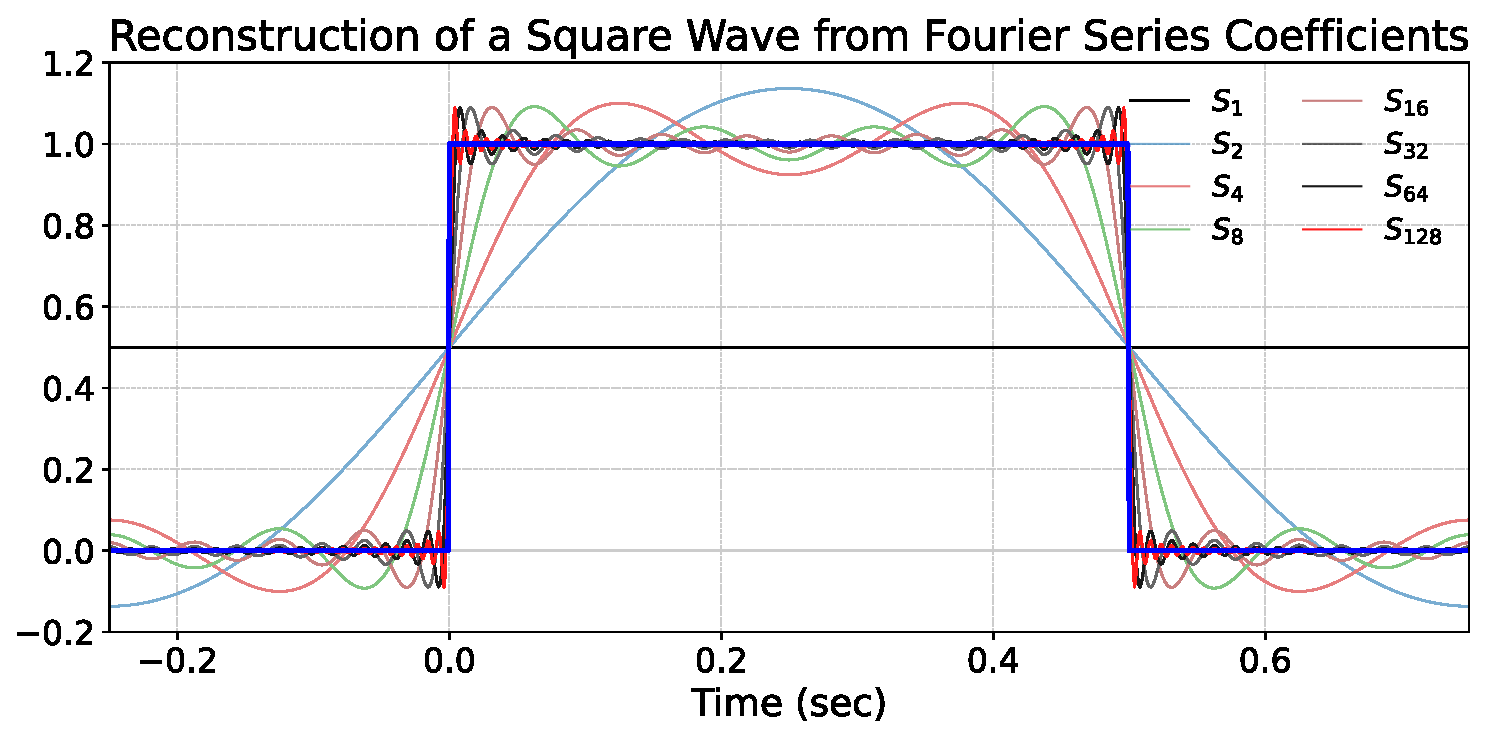
\includegraphics[width=0.8\textwidth]{img/fs-sqwave.eps}
  \end{figure}
\end{frame}


\begin{frame}[t]{Dirichlet conditions for Fourier series}
The \textit{Dirichlet conditions} guarantee that the $c_k$ exists, and $\sum_{k=-N}^{N} c_k e^{j2\pi k f_0 t}$ is equal to $x(t)$ except at time points where there is a discontinuity.
\vspace{0.5cm}

At a discontinuity, $\sum_{k=-N}^{N} c_k e^{j2\pi k f_0 t}$ converges to the midpoint of the discontinuity.
\vspace{0.5cm}

The \textit{Dirichlet conditions} are that a single cycle of $x(t)$:
\begin{enumerate}
  \item has a finite number of disconuities.
  \item has a finite number of maxima and minima.
  \item is absolutely integrable.  $\int_{0}^{T_0} \vert x(t) \vert dt < \infty$
\end{enumerate}
\end{frame}


\begin{frame}[t]{Power Spectral Density of Periodic Signals}

\textbf{Some definitions:}
\vspace{0.1cm}
\begin{itemize}
  \item Instantaneous power of a signal $x(t) \, \triangleq \, \vert x(t) \vert^2$
  \vspace{0.25cm}

  \item Total energy of a signal $x(t)$ in a time interval $[T_1, T_2] \, \triangleq \, \int_{T_1}^{T_2}\vert x(t) \vert^2 dt $
  \vspace{0.25cm}

  \item Average power over a time interval $[T_1, T_2] \, \triangleq \, \frac{1}{T_2 - T_1}\int_{T_1}^{T_2}\vert x(t) \vert^2 dt $

  \item \textbf{Energy signal}: Signals with a finite total energy and zero average power over their entire duration.
  \[ \int_{-\infty}^{\infty} \vert x(t) \vert^2 dt < \infty \quad \text{and} \quad \lim_{T \to \infty} \frac{1}{2T}\int_{-T}^{T} \vert x(t) \vert^2 dt = 0 \]

  \item \textbf{Power signal}: Signals with a finite average power, and infinite energy.
  \[ \lim_{T \to \infty} \int_{-T}^{T} \vert x(t) \vert^2 dt = \infty \quad \text{and} \quad \lim_{T \to \infty} \frac{1}{2T}\int_{-T}^{T} \vert x(t) \vert^2 dt < \infty \]
\end{itemize}
\end{frame}


\begin{frame}[t]{Power Spectral Density of Periodic Signals}
\vspace{0.25cm}

\textbf{Parseval's Identity}.
\vspace{0.25cm}

Let $x(t) = \sum_{k=-\infty}^{\infty} c_k e^{jk\omega_0t}$, then
\[ P_x = \frac{1}{T_0} \int_{0}^{T_0} \vert x(t) \vert^2 dt = \sum_{k=-\infty}^{\infty} \vert c_k \vert^2 \]

\vspace{0.5cm}

Fourier series representation preserves the average power of the periodic signal $x(t)$.

\vspace{0.5cm}

$\vert c_k \vert^2$ is the power in ofn the $k^{th}$ harmonic.

\vspace{0.5cm}

$\vert c_k \vert^2$ as a function of $k$ is the \textbf{Power Spectral Density} of $x(t)$.
\end{frame}


\begin{frame}[t]{Power Spectral Density of Periodic Signals}

\begin{figure}
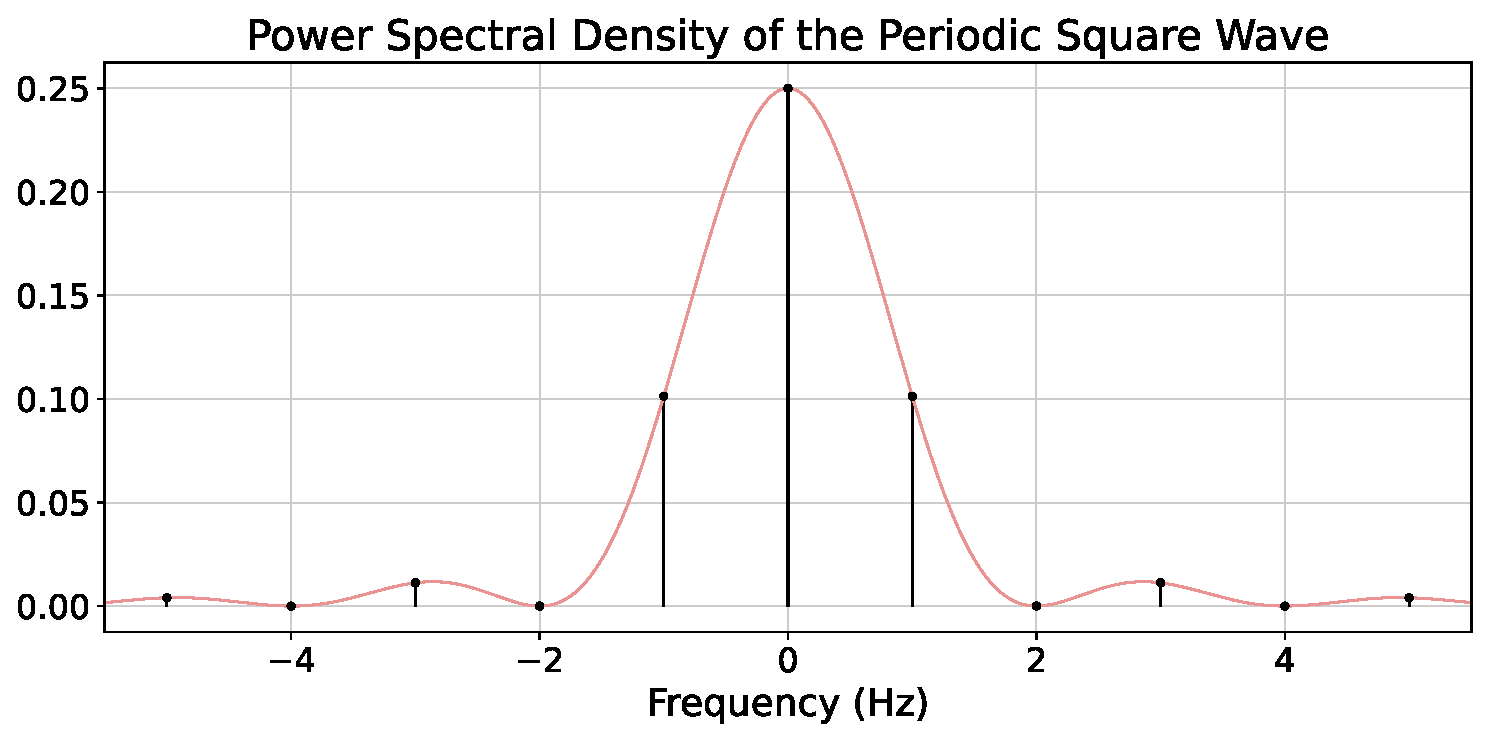
\includegraphics[width=0.8\textwidth]{img/fs-sqwave-psd.eps}
\end{figure}
\end{frame}


\begin{frame}{Power Spectral Density of Periodic Signals}
  \begin{figure}
  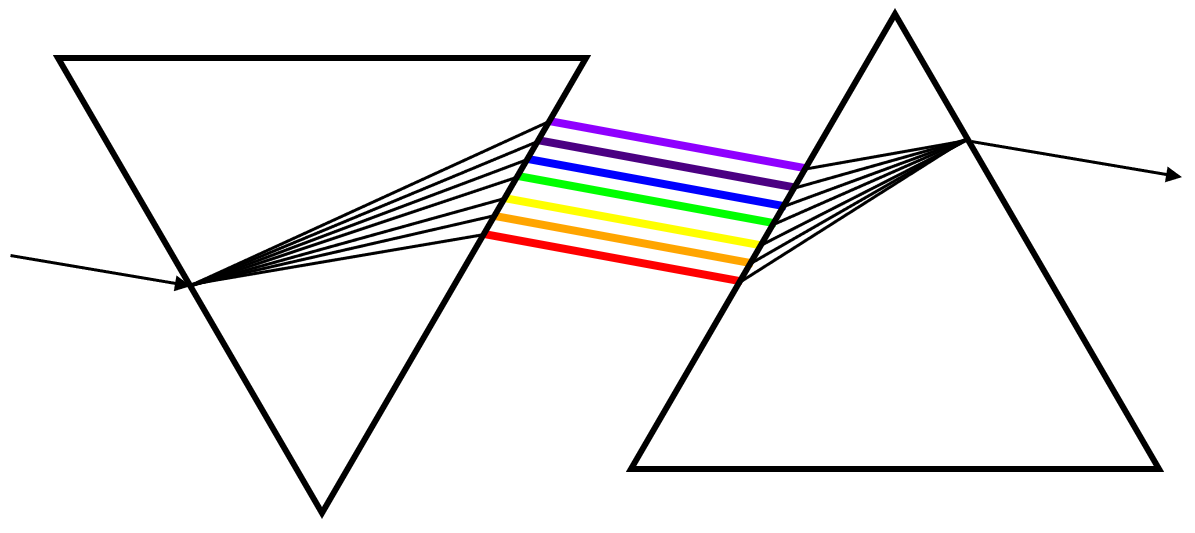
\includegraphics[width=0.8\textwidth]{img/decomp.png}
  \end{figure}
\end{frame}


\begin{frame}{Fourier representation of aperiodic signals}

We can approach this problem starting from the Fourier series.

\[ x(t) = \begin{cases}
1, & \vert t \vert \leq \frac{\tau}{2} \\
0, & \tau < \vert t \vert \leq \frac{T_0}{2} 
\end{cases}, \text{where, } 0 < \tau < \frac{T_0}{2} \]
\[ \Big\downarrow \]
\[ c_k = \frac{\tau}{T_0} \frac{\sin\lp \pi k f_0 \tau\rp}{\pi k f_0 \tau}, \,\, k = 0, \pm 1 , \pm 2, \ldots \]

\end{frame}


\begin{frame}{Fourier representation of aperiodic signals}
\begin{figure}
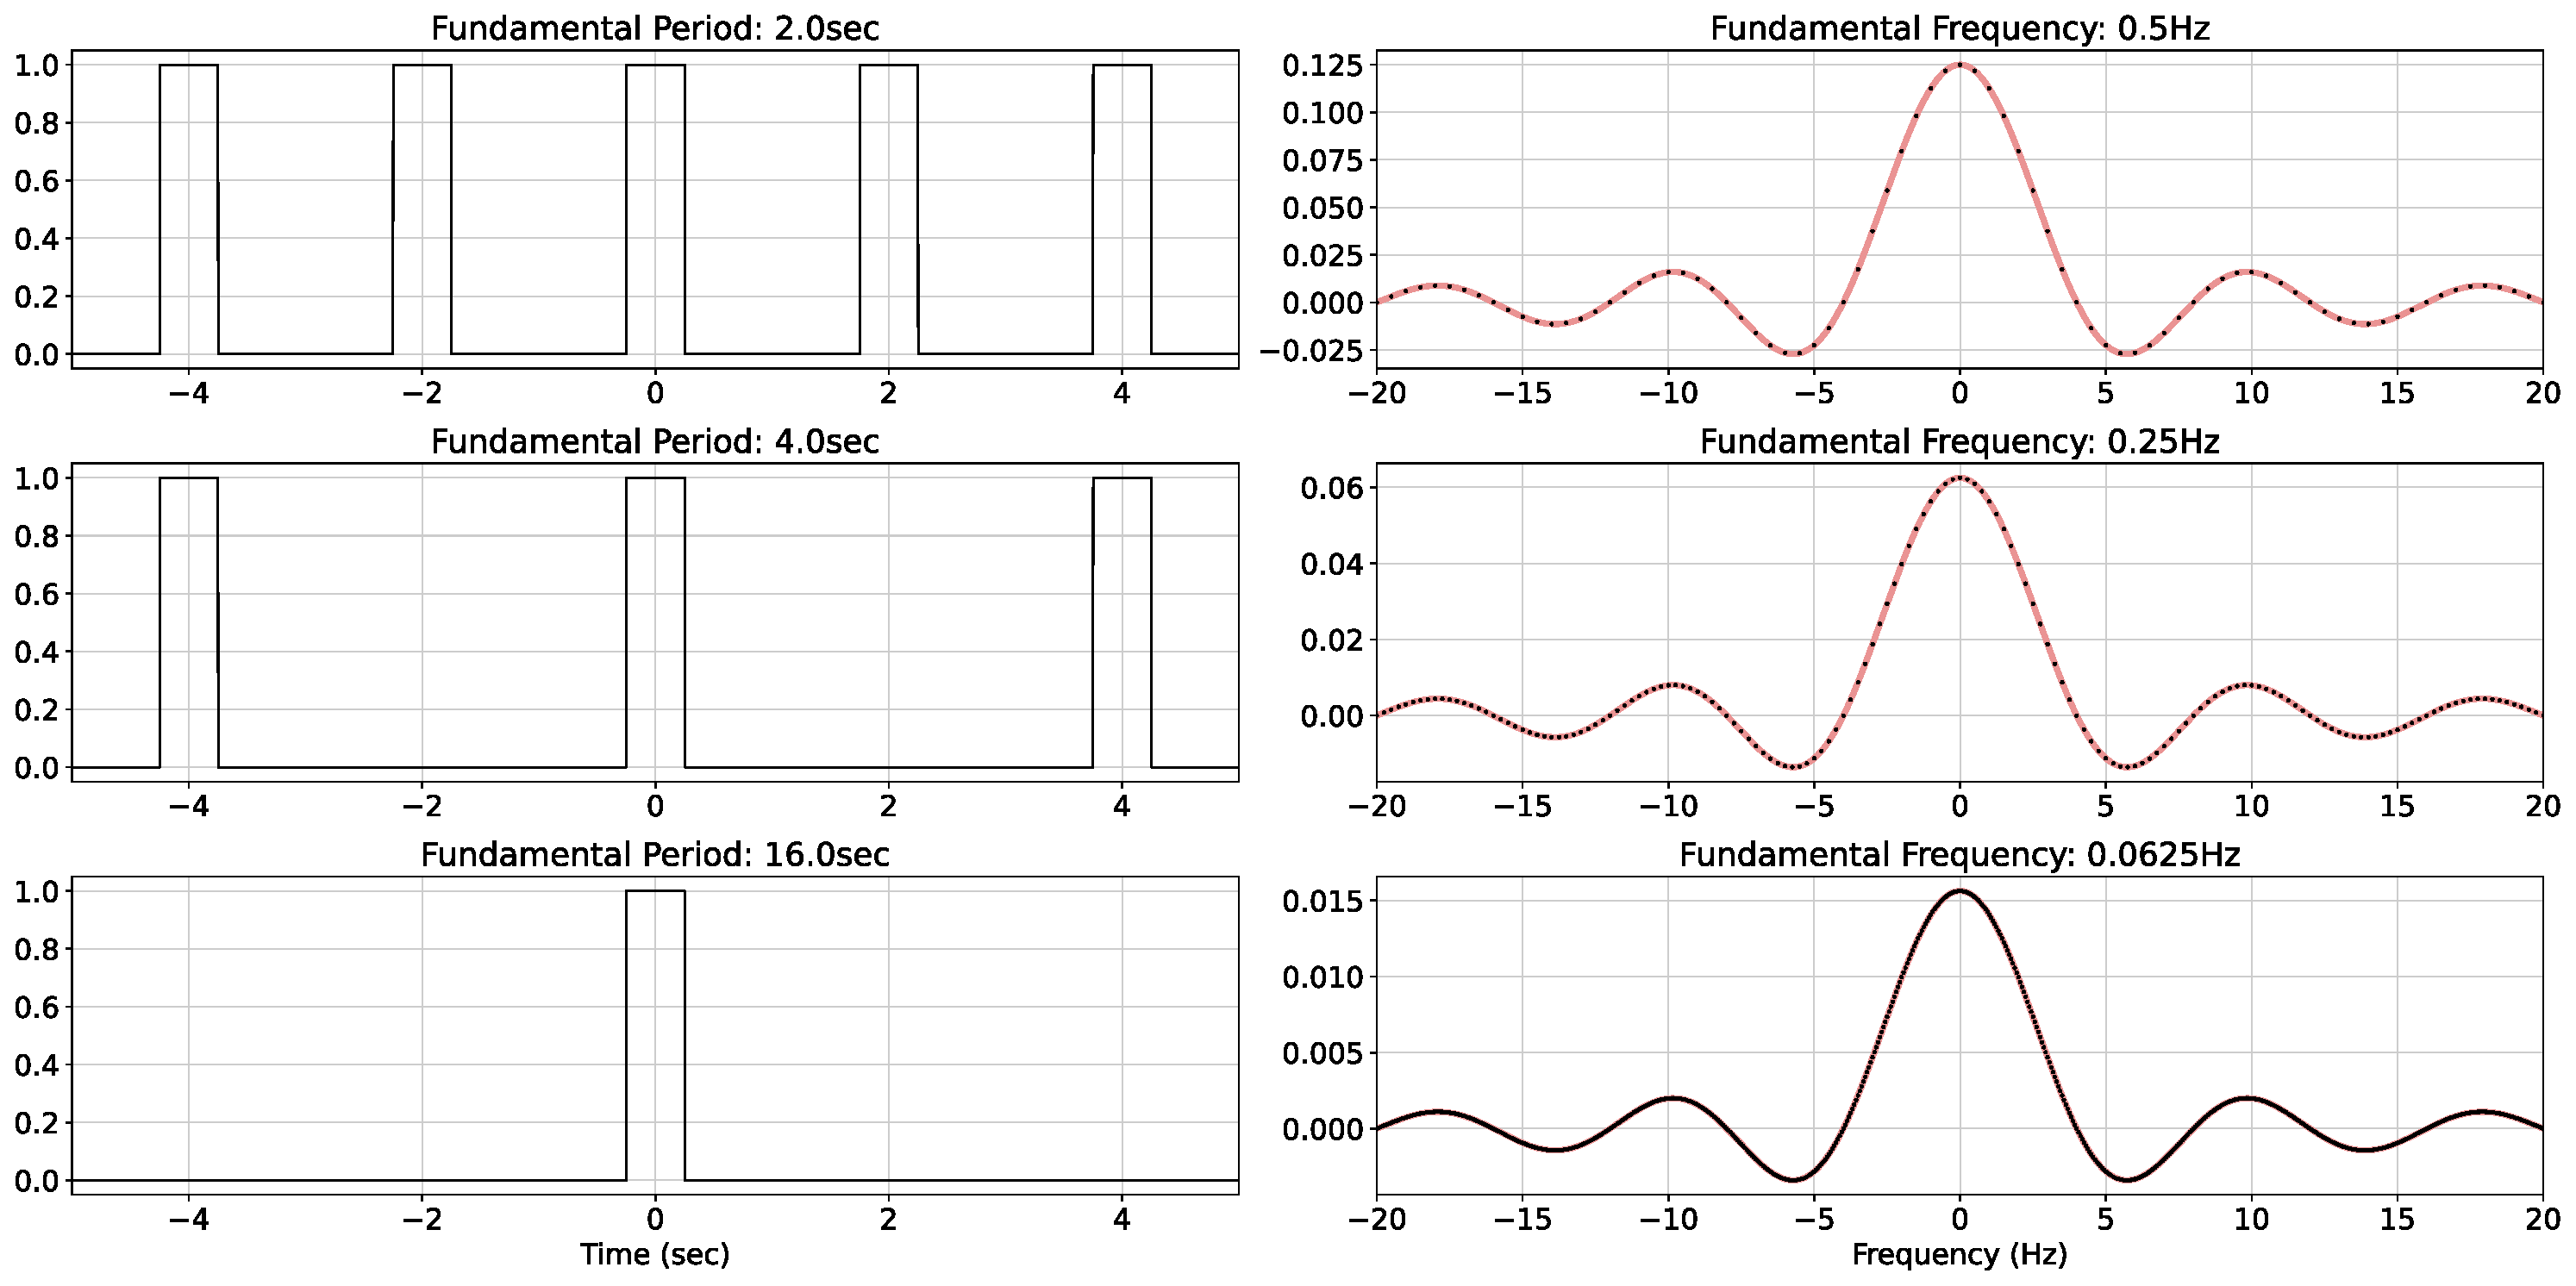
\includegraphics[width=1.0\textwidth]{img/fs-cont.eps}
\end{figure}
\end{frame}


\begin{frame}[t]{Fourier representation of aperiodic signals: Fourier Transform}
\begin{small}
\[ x(t) = \begin{cases}
1, & \vert t \vert \leq \frac{\tau}{2} \\
0, & \tau < \vert t \vert \leq \frac{T_0}{2} 
\end{cases}, \text{where, } 0 < \tau < \frac{T_0}{2} \]
\[ \Big\downarrow \]
\[ c_k = \frac{\tau}{T_0} \frac{\sin \lp \frac{k \omega_0 \tau}{2} \rp}{\frac{k \omega_0 \tau}{2}}, \,\, k = 0, \pm 1 , \pm 2, \ldots \]
\end{small}

\[ T_0 \to \infty \quad \implies \quad \omega_0 \to 0 \quad \implies \quad \left\{ k \omega_0 \right\}_{k=-\infty}^{\infty} \to \omega \in \mb{R} \quad \implies \quad c_k \to X\lp \omega \rp \]

\[ c_k = \frac{1}{T_0} \int_{0}^{T_0} x\lp t \rp e^{-jk\omega_0 t} dt \quad \longrightarrow \quad X\lp \omega \rp = \int_{-\infty}^{\infty} x\lp t \rp e^{-j\omega t} dt \]
\vspace{0.2cm}

This is the \textbf{Fourier transform}.
\end{frame}


\begin{frame}[t]{Fourier representation of aperiodic signals}
\[ x(t) = \begin{cases}
1, & \vert t \vert \leq \frac{\tau}{2} \\
0, & \frac{\tau}{2} < \vert t \vert 
\end{cases} \quad \longrightarrow \quad X\lp \omega \rp = \tau \cdot \frac{\sin\lp \frac{\omega \tau}{2} \rp}{\frac{\omega \tau}{2}} = \tau \cdot \mathrm{sinc}\lp \frac{\omega \tau}{2} \rp \]
\vspace{0.2cm}

We can reconstruct the time-domain signal from the $X\lp \omega \rp$,
\[ x(t) = \frac{1}{2\pi} \int_{-\infty}^{\infty} X\lp \omega \rp e^{j\omega t} d\omega \]
\vspace{0.2cm}

This is the \textbf{Inverse Fourier Transform.}

\end{frame}


\begin{frame}[t]{Fourier Transform}
\begin{figure}
  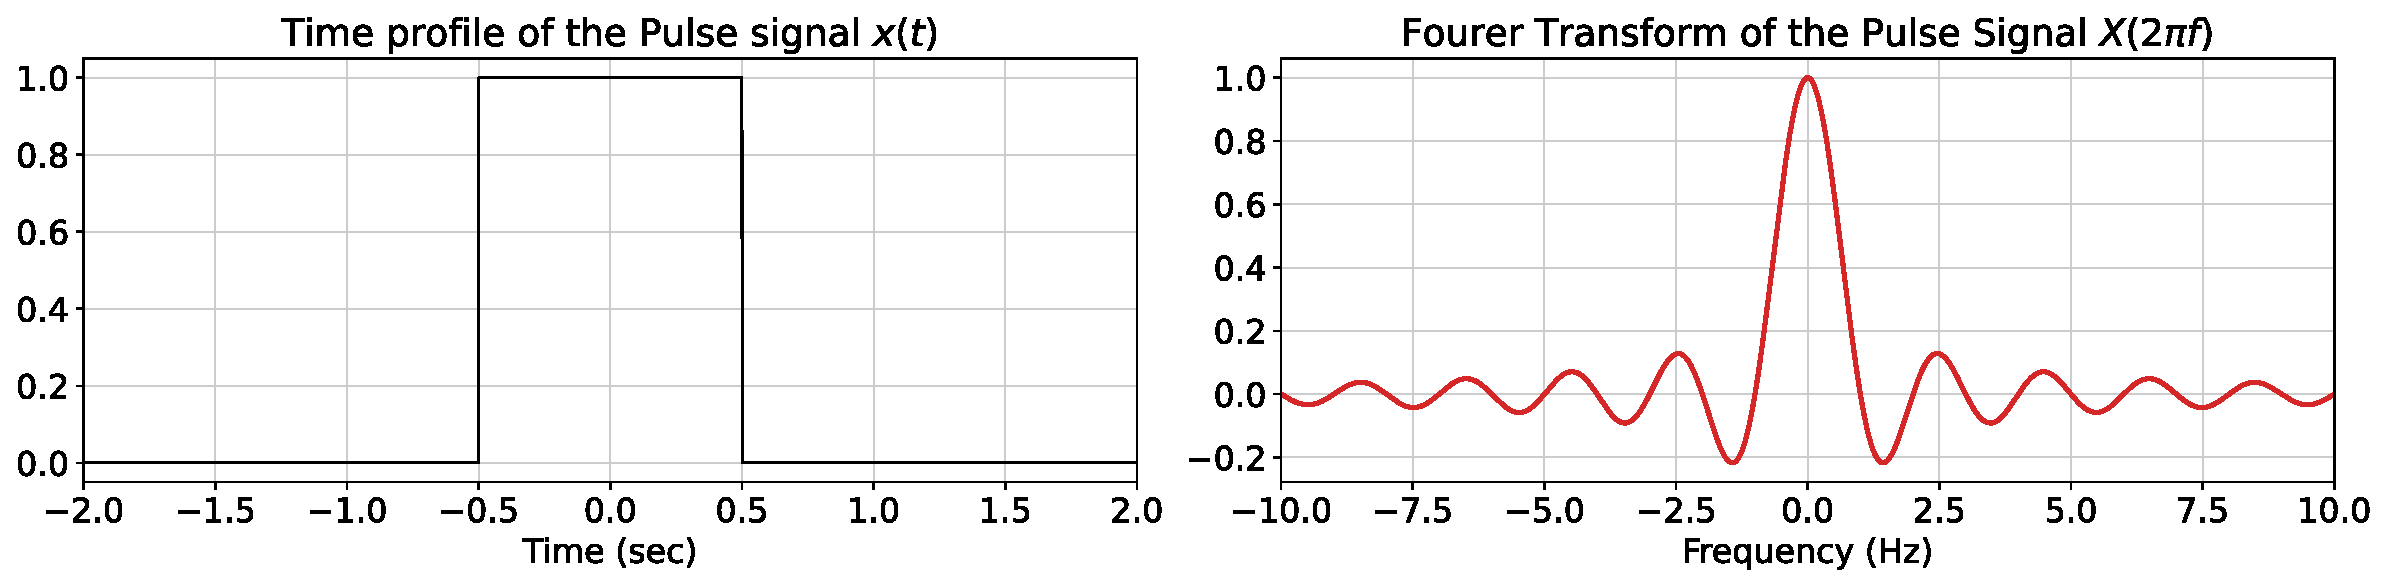
\includegraphics[width=\textwidth]{img/ft-pulse.eps}
\end{figure}
\end{frame}


\begin{frame}[t]{Fourier Transform}
\begin{figure}
  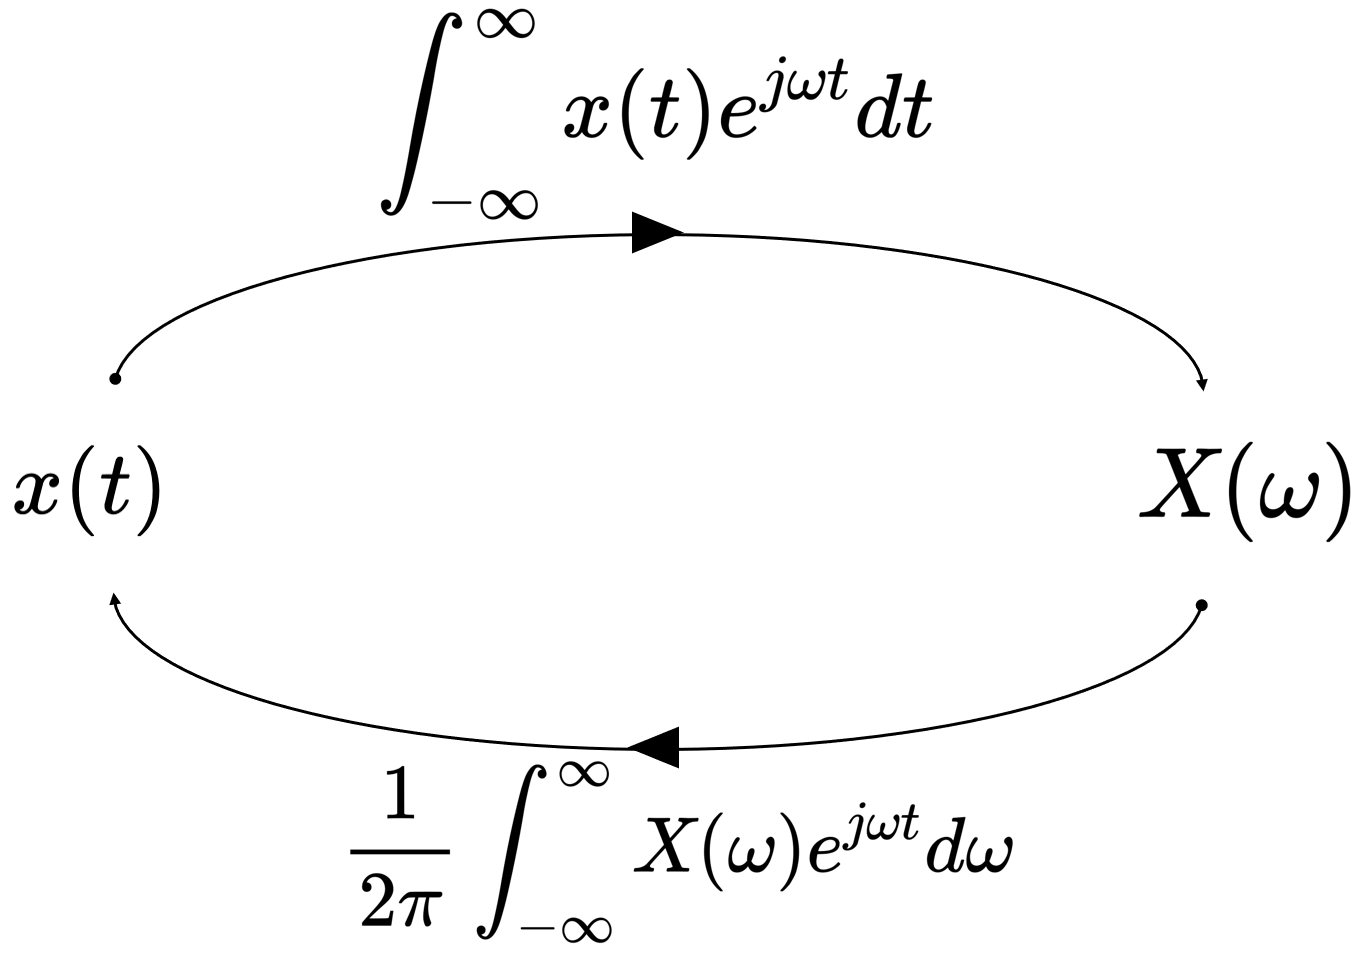
\includegraphics[width=0.7\textwidth]{img/fouriertransform.png}
\end{figure}
\end{frame}


\begin{frame}[t]{Dirichlet Conditions for the Fourier Transform}
The \textit{Dirichlet conditions} for the existence of the Fourier transform are that $x(t)$:
\begin{enumerate}
  \item has a finite number of discontinuities.
  \item has a finite number of maxima and minima.
  \item is absolutely integrable. $\int_{-\infty}^{\infty} \vert x(t) \vert dt < \infty$. 
\end{enumerate}
This ensures that $X\lp \omega \rp$ is finite and continuous.

\vspace{0.5cm}

We can still have Fourier transform for signal that are not absolutely integrable, but square integrable, i.e. $\int_{-\infty}^{\infty} \vert x(t) \vert^2 dt < \infty$.

\vspace{0.5cm}

\textbf{Example:} $x\lp t \rp = \omega_0 \mathrm{sinc}\lp \omega_0 t\rp$ is not absolutely integrable, but $X\lp \omega \rp = \begin{cases} 1, & \vert \omega \vert < \omega_0 \\ 0, & \vert \omega \vert > \omega_0\end{cases}$.
\end{frame}

\begin{frame}[t]
  \frametitle{Parseval's identity for aperiodic signals}

  Energy of an aperiodic signal $x(t)$:
  \[ E_x = \int_{-\infty}^{\infty} \vert x(t) \vert^2 dt \]

  Parseval's identity:
  \[ E_x = \int_{-\infty}^{\infty} \vert x(t) \vert^2 dt = \frac{1}{2\pi}\int_{-\infty}^{\infty} \vert X\lp \omega \rp\vert^2 d\omega \]
  
  $S_{xx}\lp \omega \rp = \frac{1}{2\pi}\vert X\lp \omega \rp\vert^2$ is the distribution of signal energey over frequency: \textbf{Energy density spectrum}.

\end{frame}


\begin{frame}{Properties of Fourier transform}

\begin{itemize}
\item \textbf{Linearity}: $\alpha x(t) + \beta y(t) \xleftrightarrow{\text{FT}} \alpha X(\omega) + \beta Y(\omega)$
\item \textbf{Shift in time}: $ x(t-t_0) \xleftrightarrow{\text{FT}} e^{-j\omega t_0}X(\omega)$
\item \textbf{Shift in frequency}: $ x(t)e^{j\omega_0 t} \xleftrightarrow{\text{FT}} X(\omega - \omega_0) $
\item \textbf{Time and frequency scaling}: $ x(\alpha t) \xleftrightarrow{\text{FT}} \frac{1}{\alpha} X\left(\frac{\omega}{\alpha}\right), \,\, \alpha > 0 $
\item \textbf{Convolution in time}: $x(t) * y(t) \xleftrightarrow{\text{FT}} X(\omega)Y(\omega) $
\item \textbf{Convolution in frequency}: $x(t) \cdot y(t) \xleftrightarrow{\text{FT}} X(\omega) * Y(\omega) $
\end{itemize}
\end{frame}


\end{document}
